\chapter{Background}\label{chap:Background}
In this chapter, we will get to know about the programming model that we follow and language syntax used in this paper. We start with the breif introduction of PGAS programming model then we will see one PGAS implementaions in Fortran language. 
\section{PGAS model}
Programming models are referenced as the style of programming where execution is invoked. In parallel computing, the programming model often expose features of hardware in order to achieve high performance. In such way, programming models in high performance computing define both the storage of data and the way data are munipulated and the way programs executed and collaborated. We defined the term of how data is stored and referenced as memory model, and how tasks are organized and  executed as execution model. 

In last few decades, people defined several parallel programming models to help abstract the parallel computing system interfaces. Given the broad variety of architectures, obviously, many different programming models have been proposed to represent features of underlying parallel machines and memory architectures. 

There are several literatures distinguishing existing popular programming models\cite{kasim2008survey}\cite{diaz2012survey}. In general, we can classify the most popular parallel programming model into three catergories:
\begin{itemize}
\item Data Parallel Model. Multiple threads execute the same instructions on different data. We note this term is often used in GPU-related loop-level parallelism.
\item Shared Memory Model. Multiple threads execute their own instruction streams, with the access to the same shared memory space. This programming model implies a convinient way for threads to communicate via data in same memory space. However, the problem behind this model is also obvious. The scalability is greatly determined by the data affinity and reference locality. Shared memory model usually use the fork-join model for execution. 
\item Distributed Memory Model. Multiple threads execute their own instruction streams, and they can only access to data in their own memory space. So the basic execution unit for distributed memory model is process with distinct memory space. The communiation between processes is carried by message passing. Distributed memory model usually deploy the Single Program Multiple Data execution model for executing the entire program. 
\end{itemize}

In general, different programming models represent different abstraction of physical system. How well the performance we can achieved by deploying certain programming model is determined by how well it matches with the underlying system. 

The Partitioned Global Adress Space(PGAS), as shown in figure~\ref{fig:pgasmodel}programming model we follow in this thesis, is consider to suit shared and distributed memory parallel machines\cite{parallelencyclopedia}\cite{stitt2009introduction}\cite{yelick2007productivity}. Ideally this programming model marries the performance and data locality (partitioning) features of distributed memory mocal with the programmability and data referencing simplicity of a shared-memory (global address space) model. 
\begin{figure}
\centering
\label{fig:pgasmodel}
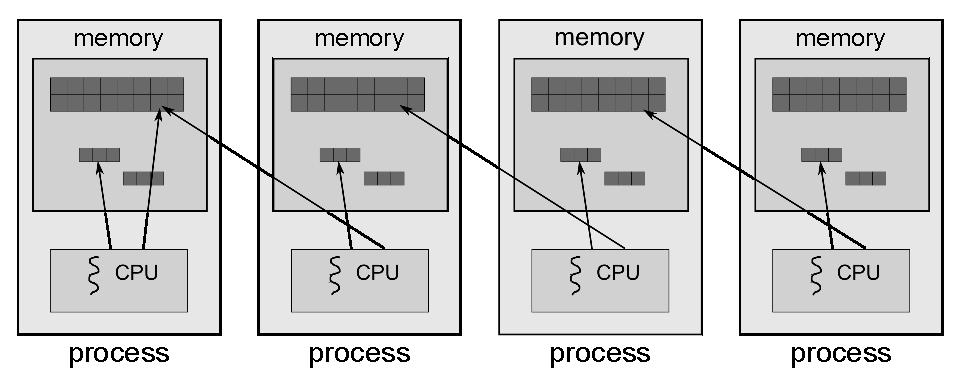
\includegraphics[scale=0.9]{figures/PGASdemo}
\caption{PGAS programming model}
\end{figure}
A system follows the PGAS programming model is expected to have following features:
\begin{itemize}
\item A set of programming unit, maybe referenced as ``threads'', ``images'' or ``Processing element'' in different implementations. Each unit has local memory storage attached to it.
\item A mechanism for each unit to share at least part of its memory space for other unit to access. 
\item Every shared memory location has explicit affinity to certain unit. 
\end{itemize}

Different from the message passing programming model, where remote data accesses between two processes requires both sides actively participating in the same communication(refered as ``two-sided communication), the PGAS programming model employs the one-sided manner. In one-sided communiation, a process can update or interrogate the memory of another process without any intervention from the destination process. On the other hand, comparing with the shared memory model, the model exposes its data affinity. In other words, the program is aware aware of where its data objects reside in relation to the one or more processing entities that are executing.

Trend in large scale computers shows the system will be based on distributed memory platform which contains much more nodes compared with today's computer system. Meanwhile each node is transforming from multi-cores to many-cores. With the growth of core count, both pure share-memory model and distributed memory model will meet their constraints in scalibility. Parallel languages and library which use PGAS programming model could potentially offer the sacalable performance both between the nodes and within the node. 

\section{Fortran in HPC}

Fortran is a high-level programming language that is wildly used in scientific programmings. The language is a procedural, imperative, compiled language with a syntax well suited to a direct representation of mathematical formulae. Individual procedures may either be grouped into modules or compiled separately, allowing the convenient construction of very large programs and of subroutine libraries. Fortran contains features for array processing, abstract and polymorphic data types, and dynamic data structures.Compilers typically generate very efficient object code, allowing an optimal use of computing resources.It is an old but still dominant base language in High Performance Computing(HPC) area. 

The history\cite{fortranlanguage} of Fortran language, which is an acronym derived from FORmula TRANslation, dates back to 1953. In the first version of Fortran, it contains several early form of construct that we can found in every high-level language, including the simple variable, assignment statement, DO-loop and etc. In following two decades, the Fortran language kept evolving until a new revision was published in 1978,  becoming known as FORTRAN 77. This standard eventually gave Fortran the position as most wildly used scientific programming language. 

Fortran always plays its important role in the area of numerical, scientific, engineering, and technical applications. And the the ISO committee ISO/IEC JTC1/SC22 /WG5 (or simply WG5) keeps this language up to date and serve the scientific programmers' needs. They have proposed a new standard which is known as Fortran 90. The main enhancement they have introduced to this version is array operations. This standard was formed at the age of supercomputer and vectorized code. This version is designed with the consideration of optimizations. The array operations, array assignments, array section and intrisic procedures for array benefit the users of this language in terms of shorter and cleaner code, reliable executable.  

Following the publication of Fortan 90 standard, a minor revision was under construction, which became what we called Fortran 95. Since it only add several changes to the Fortran 90, the mostly wild used Fortran standard is called Fortran 90/95. At the same time, the High-Performance Fortran Forum(HPFF) was formed. 
 
As the name has implied, the HPFF spent their effort in making extensions to Fortran language to produce portable, single-threaded code working in parallel machines. This work is called High Performance Fortran(HPF).  The HPF follows the data parallel model where the data is represented as regular grid spreading over multiple processors. This allows efficient implementation on SIMD and MIMD architectures. Given such syntax nature, they chose the Fortran 90, which has adequate array language, as the base language. HPF features includes:
\begin{itemize}
\item New Fortran statement, such as \emph{FORALL} statement for loop-level parallism
\item Directives for distribution of array data, such as 
\begin{lstlisting}
!HPF$ DISTRIBUTE A(BLOCK,*)
!HPF$ ALIGN B(I,J) WITH A(I,J)
\end{lstlisting}
\item Additionally intrinsic library routines. 
\end{itemize} 
HPF left lot of optimization opportunities for compilers. During this period, lot of papers have been published about implementation and optimization of HPF in compilers\cite{loveman1993high}\cite{bozkus1994compiling}\cite{gupta1995hpf}. Unfortunately, although HPF has engaged some interest and success at the beginning, it eventually faded away. Lesson has been learned from this parallel language experiment\cite{Kennedy2011}. However, the HPF did introduce some pioneer ideas to the HPC field. It inspired many successors including Fortran and its variants, OpenMP and many more HPC languages and it did influent the way how upcoming Fortran parallel extensions are designed. 

There are a large Fortran code demanding for speedup when no parallel feature introduced officially into the standard. Several auxiliary libraries and extensions, besides the HPF mentioned above, have been proposesd. The OpenMP and MPI, which are very famous nowaday, formalized their Fortran interfaces. Also, R. W. Numrich and J. K. Reid\cite{numrich1998co} published a paper describing their proposal of parallel extensions for Fortran called Co-Array Fortran, which has been absorded to recent Fortran language standard and its the main topic of this thesis. We will talk about the syntax of Co-Aarray Fortran later in chapter~\ref{chap:Methods}. 

It was no parallel features included into Fortran standard until Fortran 2008 is announced. In the language specification we can see those handful Co-Array syntax and some necessary intrinsic routines that come from the Co-Array Fortran extension. As they are added into the standard, several commercial compilers, including Cray compiler and Intel compiler, are supporting these features. Some acedamic groups have studied its performance and potential\cite{barrett2006co}\cite{coarfa2003co} in both acedamic benchmarks and industry prototype codebase. More auxiliary parallel features are under discussion in the draft Technical Specification TS18508 Additional Parallel Features in Fortran\cite{caf-spec}.

\section{Task Decomposition in Parallel Program}

While SPMD has been widely adopted as the programming model followed by many parallel languages, libraries and interfaces, its restrictiveness does imply some drawbacks. The pure SPMD programming model implies a relatively flat machine model, with no distinction between any execution unit that may resident in close or far-away pyhsical location. Most PGAS languages and libraries lack the capability to expose this awareness of underlying hiearchy. As consequence, the communication costs that are not transparent for users hurt the performance. Similarly, it make the PGAS model, which should be easily adopted to heterogeneous environment, become difficult to program for heterogeneous machine. Finally, SPMD programs have difficulty in performing dynamic load balancing. 

In MPI\cite{gropp1999using}, the \textit{communicator} serves as the representation of subset of processes. It enables programmers to express the potential task parallelism in problem space. There are two possible task parallelism we are going to consider in this thesis. 

The first program pattern to consider is parallel divide-and-conquer method. In classical algorithm study, the divide-and-conquer is a common method applied to take down the task size and solve them in reasonable time. In Dr.Hardwick's work\cite{hardwick1997practical}, he summerized the pratical divide and conquer method and proposed the term \textit{team parallism}. This method is data-oriented, that is, the parallel program can benefit from dividing the data into small chunk and processing them concurrently. The procedures for each \textit{team} or subset of processes are all identical. There are several example applications following this parallel programming pattern, like parallel quick sort and parallel sample sort\cite{hirschberg1978fast}. In such way, we would like a nested \textit{team} construct to better map to the underlying memory hierachy.

The second pattern is more general. In parallel programming with task paralleism, it is common for different components of an algorithm to be assigned to different units. For example, a climate simulation may assign a subset of all processes to model the atmosphere, while an other subset to tackle with the ocean model. Each of these components can in turn be decoposed into seperate parts for different purposes or algorithms. For instance, a subset such as one piece that performs a stencil while another piece could do Fourier transform. In such case, the decomposition does not directly depend on the layout of the underlying machine, although we can tell it would be benefit to assign threads nears to each other into one functional team.

Lot of researchers working in PGAS field realize the need for such method to do decomposition in parallel program. Since 2012, researchers who was working on Titanium project and UPC project published their proposal to add hierarchical additions to the SPMD programming model\cite{kamil2012hierarchical}\cite{upc-teams}. They proposed the \textit{nested team} construct to express the hierarchy of underlying machines. Compared with MPI, this \textit{nested team} construct is more structural, however, it serves as an better abstraction of hiearchy, other than a general subset of processes. Later the OpenSHMEM work group\cite{shmem-teams} has proposed their \textit{team} design regarding to the task decomposition. The \textit{nested team} has been indentified as a reasonable way to carry the work.

\section{Survey of Coarray Fortran Implementations}\label{sec:survey}

Although we will not go into the details of Coarray syntax until Chapter~\ref{chap:Methods}, here we will look at some on-going compiler and library that support Coarrays. As far as we know, Cray has always been working on the lastest Fortran language features and always achieve the most efficient performance. But we can only know little detail about this commercial compiler. Here we will talk about two open-source project, from OpenCoarrays project and Rice University. 

\subsection{OpenCoarrays}
OpenCoarrays\cite{opencoarrays} is an open-source software project that produces an application binary interface (ABI) supporting coarray Fortran (CAF) compilers, an application programming interface (API) that supports users of non-CAF compilers, and an associated compiler wrapper and program launcher.

OpenCoarrays is not a module for a particular compiler. It is a portable translation layer that supposed to convert Coarray syntax to an abstract API that should adapt to any non-CAF compiler later on. Right now it works with GNU Fortran compiler(gfortran). It supports Coarray syntax introduced in Fortran 2008, and some features in Technical Specification. As when we look into their source code, it shows they still need more optimization work on the to-do list. 

\subsection{Rice CAF 2.0}\label{sec:caf2.0}
The research group in Rice University started their supporting of Coarrays in an early stage\cite{dotsenko2004multi}. They have implemented a prototype of an open-source, multiplatform CAF compiler that generates code for most common parallel architecture. The cafc compiler translates CAF into Fortran 90 plus calls to one-sided communication primitives, which can further be mapped to certain communication layer library calls. In this implementation, they have supported Coarray descriptor, shared memory object management,  translating coarray assignemnt to communication calls and some intrinsic procedures. Basically, the first version of cafc compiler supported most syntax mentioned in Fortran 2008. 

Soon after, the research group found the shortage of functions these syntax can provide to user. In publication\cite{mellor2009new} after the announcement of Fortran 2008 standard, they summerized what they think are missing in this extension as following.
\begin{itemize}
\item There is no support for processor subsets
\item The coarray extensions lack any notion of global pointers
\item There is no support for collective communication
\end{itemize}

To address these shortcomings, Rice University is developing a redesign of the Coarray Fortran programming model. Rice's new design for Coarray Fortran, which is call Coarray Fortran 2.0, is an set of coarray-based extensions to Fortran designed to provide a different parallel programming model. Compared to the emerging Fortran 2008, Rice's new coarray-based language extensions include some additional features:
\begin{itemize}
\item process subsets known as teams, which support coarrays, collective communication, and relative indexing of process images for pair-wise operations, 
\item topologies, which augment teams with a logical communication structure,
\item dynamic allocation/deallocation of coarrays and other shared data,
\item team-based coarray allocation and deallocation, global pointers in support of dynamic data structures, \item enhanced support for synchronization for fine control over program execution,
\end{itemize}

Rice's implementations of Coarray Fortran 2.0 has the similiar way as we have implemented Fortran 2008. The compiler would translate the Coarray Fortran program to Fortran90/95 program with calls to runtime library primitives. 

Although the group claim the Coarray Fortran 2.0 is still a progressing work, they have switched their focus to hierarchical PGAS or APGAS. \textit{Team} also show in context but in a little different manner. 
